\documentclass[12pt]{article}
\usepackage{sbc-template}
\usepackage{graphicx,url}
\usepackage[export]{adjustbox}
\usepackage[latin1,utf8]{inputenc}
\usepackage[nottoc]{tocbibind}
\usepackage[T1]{fontenc}
\usepackage[portuguese]{babel}
\usepackage{hyphenat}
\hyphenation{mate-mática recu-perar}

\graphicspath{{img/}}

\sloppy

\title{Projeto de Engenharia de Software \\ UP! SHARING}

\address{Instituto de Informática - Instituto de Pesquisas Tecnologicas do Estado de São Paulo (IPT)\\ Caixa Postal 15.064 - 91.501-970 -- São Paulo -- SP -- Brazil}

\author{Alex A. Prado\inst{1}, Dirce Mudrai\inst{1}, Ivan Borges\inst{1} \email{alex.azprado@gmail.com, dirce.mudrai@icloud.com,
  ivangb@gmail.com}}

\begin{document} 

\maketitle

\begin{abstract}

This software engineering project, which will be available for mobile devices, with access to the cloud infrastructure aims to meet a need for the automaker provide car sharing for a specific line of vehicles, widely used in shared lease. This type of rent allows several economic, social and environmental gains.
 
\end{abstract}
     
\begin{resumo} 

Esse projeto de engenharia de software, que estará disponível para dispositivos móveis, com acesso à infraestrutura em nuvem visa suprir uma necessidade da montadora em fornecer serviço de locação para uma linha específica de veículos. Este tipo de locação possibilita diversos ganhos econômicos, sociais e ambientais. 
Os requisitos deverão ser os funcionais e não funcionais, deixando claro quais são seus objetivos. Deve permitir desde já a sua rastreabilidade, bem como descrever os  atores. Elaborar um modelo de processo que contemple as necessidades de configuração.
Os itens de qualidade devem ser considerados quanto às funcionalidades   e tempos de resposta.
Um modelo conceitual deverá ser feito, utilizando a notação UML – \textit{Unified Modeling Language}, com seus respectivos diagramas, fluxos de dados e interações.
Deve-se já em tempo de levantamento de requisitos, derivar uma solução de arquitetura do sistema.
Os possíveis conflitos entre dois usuários, devem ser resolvidos através de negociação entre as partes. 
Por se tratar de um sistema de desenvolvimento de software complexo, um plano de risco deverá ser elaborado. 
A prototipação deverá ser elaborada a fim de validar os requisitos elicitados e levantados.
Deverá ser considerado como serão feitos os testes de aceite, visando o produto final.
Descrever as regras para eventuais mudanças nos requerimentos, elaborando uma Gestão de Mudanças.
Quanto às ferramentas para as diversas atividades citadas será utilizado o que a empresa já utiliza no momento.

\end{resumo}


\section{Introdução ao Projeto}



Entende-se locação compartilhada (CAR SHARING) como a forma de utilização comunitária de um mesmo veículo como meio de transporte dada a sua disponibilidade. Este termo é utilizado para definir um modelo de aluguel de veículos em que o cliente aluga o carro para uma quantidade específica ou para uso rápido, com um conceito de autos serviço, em que o cliente é independente e autônomo na utilização do serviço.

\section{Condições e características importantes}

vamos fazer ainda

\section{Disciplinas do SWEBOK}
\subsection{Requisitos}

Estão envolvidos no processo os usuários finais, a fabricante dos veículos e a empresa locadora. Deve-se criar um comitê de representantes da locadora e do fabricante que irá interagir com um grupo de usuários convidados. Assim, os requisitos atenderão a todos os envolvidos, conforme o SWEBOK \cite{Swebok}.
Quanto aos requisitos, será necessário elicitá-los, detalhá-los junto com dois tipos de usuários: aqueles que utilizarão o sistema e aqueles que tratarão da parte financeira. J. Fowlkes \cite{Fowlkes2000} propõe uma forma de elicitação de requisitos por vídeo, e vem de encontro ao propósito desse trabalho, principalmente gravando nos diversos estacionamentos e locais de locação, cujos requisitos serão elencados utilizando o método descrito em seu artigo.
Assumindo a característica de inovação do projeto, bem como sua proposta de integração com o meio ambiente, o mesmo deverá preparar-se para a interoperabilidade com sistemas de iluminação de ruas efetuando a gravação de imagens durante o percurso dos carros e fazendo a identificação da iluminação presente. Seguindo o processo de Pooya \cite{Pooya}, as imagens poderão ser capturadas, processadas e transmitidas para os provedores de sistemas de iluminação, otimizando os custos de manutenção da rede. A ideia principal pode ser visualizada na figura \ref{fig:exampleFig1}. Dessa maneira, ele pode transmitir para a companhia de energia, quais luzes estão queimadas, não tendo custo de manutenção, integrando junto à comunidade que ele atua. Com isso a  Volkswagem poderá reunir benefícios à marca.

\begin{figure}[htp]
\centering
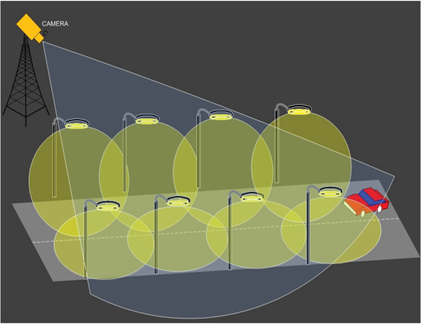
\includegraphics[scale=.8] {swebok_requisitos.png}
\caption{Monitoração remota com visão computadorizada}
\label{fig:exampleFig1}
\end{figure}

\subsection{Desenho do Software}

Para desenhar o Sistema Volkswagen up! Sharing, utilizaremos uma arquitetura de software orientada a serviços \textbf{SOA} - \textit{Service Oriented Architecture} de forma a se ter um padrão, (hoje muitos deles já existente na organização) que seja possível a interoperabilidade e reuso de aplicações, independentemente de linguagens e plataformas de hardware ou software, que é uma diretriz da área de TI da Volkswagen. Conforme salienta Niemann \cite{Niemann2008}, quanto ao ciclo de vida SOA, nosso propósito é utilizar tal ciclo de vida. 
Deverá ter uma visão estática e dinâmica conforme o SWEBOK \cite{Swebok}, utilizando a notação UML com a ferramenta que a empresa oferece.


\subsection{Construção de Software}

Dado a complexidade do sistema Volkswagen up! Sharing optamos por uma construção de metodologia de desenvolvimento Iterativo e incremental, cujas vantagens foram demonstradas por Eduardo Bezerra \cite{Bezerra}.
O sistema será desenvolvido na linguagem JAVA e deverá ser desenvolvido de forma a atender os sistemas operacionais ANDROID e IOS.
Os testes isolados serão feitos nessa fase, conforme SWEBOK \cite{Swebok}

\subsection{Teste de Software}

Para a execução dos testes  do sistema VOLKSWAGEN UP! SHARING, adotaremos testes dinâmicos  e testes finitos, dentro de critérios de seleção, conforme SWEBOK \cite{Swebok}. Para isso seguiremos ao exposto por I. Journal \cite{Journal2013}, onde em seu item 2 – \textit{Material and Methods}, aborda os testes para atender aos requisitos do sistema.

Como trata-se de um sistema que deve contemplar dois tipos de usuário: aquele que se utilizará do sistema e a parte financeira, conforme descrito no item 3.1 Requisitos, separaremos esses testes nas duas partes citadas, porém com o mesmo ciclo de vida, ou seja, haverá o \textit{Teste Life Cycle} para a parte financeira e outro \textit{Teste Life Cycle} para o propósito do sistema VOLKSWAGEN UP! SHARING seja avaliado pelos usuários finais seguindo as seguintes etapas.


TEST PLAN PREPARATION: \\
Onde temos o planejamento dos testes, como um Road Map, identificando todas as atividades dos testes. Apesar da empresa possuir ferramenta de automatização de testes, optamos por fazer os testes de requisitos funcionais manualmente a fim de garantir plenamente suas funcionalidades. \newline
Nesse planejamento teremos os testes de Caminho Básico, conforme Pressman \cite{Pressman}, bem como a complexidade ciclomática, nos mostrando os caminhos independentes, garantindo dessa forma que todas as instruções foram executadas pelo menos uma vez. 
Além disso, os testes integrados, testes de regressão, aceite e stress serão planejados. \newline
Como nosso sistema também estará disponível nos celulares, tabletes, também será planejado os testes WebApp, como Pressman \cite{Pressman} nos mostra que deveremos fazer os testes de conteúdo, função, estrutura, usabilidade, navegabilidade entre outros.

TEST CASE DESIGN: \\
Processo onde selecionamos determinados dados de entrada e executamos o software numa determinada condição específica. Essas condições específicas ser apresentadas no plano \textit{Test Plan Preparation}.

TEST EXECUTION: \\
Processo de execução dos casos de testes.

TEST LOG PREPARATION: \\
Processo onde são preparados todos as possíveis saídas resultante de um conjunto de teste.

DEFECT TRACKING: \\
As falhas são rastreadas, defeito por defeito para posteriormente gerar relatórios de defeitos.

TEST REPORT GENERATION: \\
São relatórios que demostram todos os testes efetuados.


\subsection{Manutenção de Software}

O sistema utilizará um framework dirigido por dados e, desta maneira, de acordo com Patil 2016 (Automated Software Testing for High-end Touch Screen Automotive Displays), se beneficiará de uma manutenção facilitada, já que será possível encontrar quais scripts contém componentes comuns para serem atualizados. Ainda de acordo com Patil 2016, Isto resultará num aumento da reusabilidade, proporcionando mais cenários de testes e reduzindo o tempo de desenvolvimento necessário.

Considerando-se o item anterior e o fato de o sistema necessitar de interação facilitada por parte dos motoristas, a manutenção dos eventuais defeitos do software deverão priorizar a análise de feedbacks dos usuários, como apresentam Kittiya e Pornsiri 2016 (Prioritizing Software Maintenance Plan by Analyzing User Feedback). O método em questão, apresentado na Fig.99, dispõe de 2 partes. A primeira é o processo de extração de palavras-chaves relacionadas a defeitos no software através de linguagem natural utilizando-se relações gramaticais. A segunda parte é o processo de se atribuir o ranking de impacto do defeito utilizando-se algoritmo AHP.


\begin{figure}[ht]
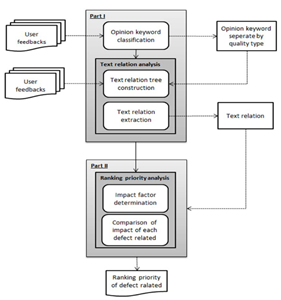
\includegraphics[scale=.8, center] {swebok_manutencao.png}
\caption{Visão Geral de priorização em Plano de Manutenção de Software por Análise de feedback de usuário}
\label{fig:exampleFig2}
\end{figure}

Por fim, com a finalidade de se reduzir termos redundantes do processo de manutenção da aplicação por análise de feedback do usuário, deverão ser utilizadas as técnicas expostas por Oscar e Andrian 2016  (On the Reduction of Verbose Queries in Text Retrieval Based Software Maintenance) que visam remover termos específicos de consultas em contextos de conceitos baseados em Busca Textual, otimizando o emprego de informação gerada pelo usuário para levantamento de possíveis erros a serem manutenidos.

\subsection{Gerenciamento de Configuração de Software}

Dada a característica crítica e de segurança desta aplicação, o gerenciamento de configuração deverá seguir os padrões aplicados pelo IEEE em seu documento 828-1983 (IEEE Standard for Software Configuration Management Plans). Isto visará o provimento de requisitos mínimos quanto à preparação e criação de conteúdo do Plano de Gerenciamento de Configuração do Software.

A ferramenta a ser utilizada neste processo será determinada de acordo com a teoria de conjunto difuso (fuzzy set) de análise. Desta maneira, a aplicação prática deste processo será a análise qualitativa e a utilização de um método de combinação calculado quantitativo, oferecendo flexibilidade na determinação do sistema de índice de avaliação e seu valor de pesos, como sugerido por Yongchang et al (Fuzzy Decision Analysis of the Software Configuration Management Tools Selection).

Desta maneira, dada a dinâmica e qualidades exigidas para o controle de compartilhamento de carros, uma escolha fundamentada desta ferramenta de gerenciamento propiciará o melhor atendimento das necessidades do sistema. Para esta escolha, ainda de acordo com Yongchang et al (Fuzzy Decision Analysis of the Software Configuration Management Tools Selection), o índice de avaliação deste quesito se resumirá à função, desempenho, custo, serviço e outros quatro fatores de primeiro nível. Dentre eles, a função terá quatro índices de nível 2, o desempenho terá três índices de nível 3. Um diagrama de hierarquia de decisão de seleção pode ser visto na figura \ref{fig:exampleFig3}

\begin{figure}[htp]
\centering
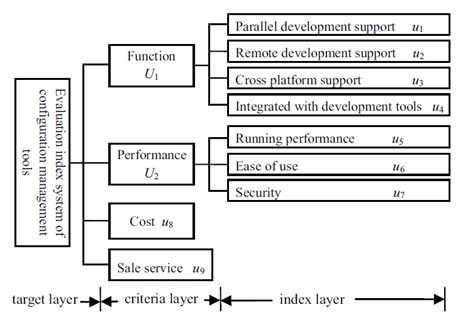
\includegraphics[scale=.8] {swebok_configuration.png}
\caption{Índice de avaliação de hierarquia de decisão de seleção de ferramentas}
\label{fig:exampleFig3}
\end{figure}


\subsection{Gerenciamento da Engenharia de Software}

Como ferramenta de Gerenciamento de Engenharia de Software para análise de metas de desempenho, utilizaremos a ferramenta “MultiPERF”, baseada no repositório de dados de projeto de software internacional ISBSG, proposto para atribuir metas de desempenho como apresentado no estudo de Vasile, Pierre e Alain 2014 (A White-Box Tool to Set Performance Targets in Software Engineering Management using the ISBSG Repository). A proposta, neste caso, se justifica pelo fato de que a ferramenta “MultiPERF”, baseada em planilhas Excel, se benefica do repositório ISBSG, que por sua vez permite análise de metas através de variadas funções. Desta maneira, procura-se assegurar aos locadores de nossos carros um desempenho satisfatório do aplicativo por eles utilizados.

Para um melhor gerenciamento da estimativa de esforços, seguiremos os conceitos expostos na publicação de Velarde et al 2016 (Software Development Effort Estimation based-on Multiple Classifier system and Lines of Code), os quais se comprometem a uma precisão de 71\% na estimativa dos esforços previstos. Dadas as características de nossa equipe de desenvolvimeno, tal qualidade propiciará uma melhor alocação de recursos e confiabilidade na tomada de decisões dentro do planejamento de desenvolvimento.

O conjunto de aplicações necessárias para implementação de todo o sistema, o qual atuará em frentes distintas para possibilitar o gerenciamento dos usuários, dos carros, das localidades onde se encontram e dos trajetos por eles percorridos demonstra um vasto leque de participantes no desenvolvimento. Desta maneira, como proposto por Farhan Sarfraz 2009 (Managing for a Successful Project Closure), o término do projeto será identificado como bem sucedido através do emprego de diretrizes que implementarão o envolvimento de toda equipe, comunicação pós-encerramento com todas as partes interessadas, atualizações regulares sobre a execução dos processos restantes. Estas diretrizes terão por objetivo o desencadeamento de um comportamento psicológico positivo de todos os membros assegurando o encerramento com êxito.


\subsection{Processo da Engenharia de Software}

De acordo com expectativas da montadora Volkswagen e seu carro Up!, carro a ser usado na frota, o software precisará ter um apelo de relacionamento com os usuários. Para que isto seja alcançado, e no que diz respeito aos processos de engenharia de software, seguiremos as diretrizes de Amal, Christian e Claude 2014 (Implementing and validating SynchSPEM A solution for synchronizing activities and products within a software engineering process), que utiliza o SynchSPEM como um modelo de metadados para monitorar a evolução do desenvolvimento de maneira a se certificar de que haja consitência e coerência na evolução do processo.
Deverá ser empregado o modelo AHAA – Agile, Hybrid Assesment Method for Automotive, definido por Fergal, Minna e Ita 2008 (AHAA –Agile, Hybrid Assessment Method for Automotive, Safety Critical SMEs) para combinar o ciclo de vida do desenvolvimento do software com um desejado aumento da qualidade do produto desenvolvido. Este método, que faz uso do “Automotive SPICE Process Reference Model, se adequa às exigências aos fornecedores da indústria automobilística no que se refere a processos de software. 

Para se adequar às imposições da indústria automotiva no que se refere à interação do usuário, a segurança operacional deverá ser levada em consideração, e para isto o processo de software seguirá imposições de agências reguladoras, objetivando um melhor monitoramento da qualidade do software através de seu desenvolvimento. Abaixo vemos a Fig.99, ainda de Fergal, Minna e Ita, ilustrando os componentes que deverão ter especial atenção para determinar uma melhor aproximação ao modelo de maturidade e atingir a avaliação desejada.

\begin{figure}[ht]
\centering
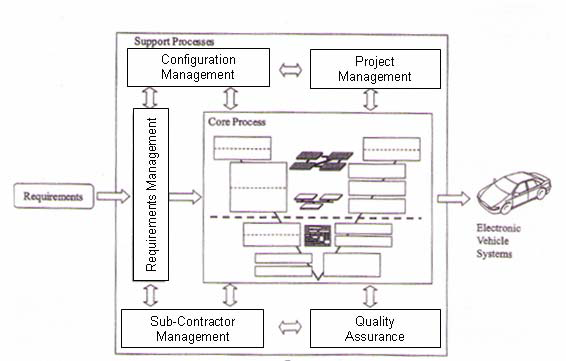
\includegraphics[scale=.7] {swebok_engenharia.png}
\caption{Processos de suporte para Sistemas Eletrônicos e Desenvolvimento de Software.}
\label{fig:exampleFig4}
\end{figure}

\subsection{Modelos e Métodos na Engenharia de Software}

O projeto UP! Sharing, será desenvolvido de maneira organizada e sistemática para garantir a entrega do produto final utilizando os métodos e ferramentas de engenharia de software adequados. 
As ferramentas da engenharia de software fornecem suporte automatizado ou semiautomatizado para o processo e para os métodos. Quando as ferramentas são integradas, de modo que as informações criadas por uma ferramenta possam ser utilizadas por outra, é estabelecido um sistema para o suporte ao desenvolvimento de software.
\cite{pressman2016engenharia}

Os métodos da engenharia de software fornecem as informações técnicas para desenvolver software. Os métodos envolvem uma ampla variedade de tarefas, que incluem: comunicação, análise de requisitos, modelagem de projeto, construção de programa, testes e suporte. Os métodos da engenharia de software se baseiam em um conjunto de princípios básicos que governam cada área da tecnologia e incluem atividades de modelagem e outras técnicas descritivas.

O método ágil para gestão de projetos apresenta um modelo mais amigável de gestão que outros por este motivo, foi definido como sendo mais adequado para o projeto. O scrum master gerencia as atividades de maneira incremental que recebe o nome de Sprint e não pode durar mais de 30 dias. A lista do Product Backlog Item (PBI) é gerada a partir das atividades que são identificadas, definidas, priorizadas e estimadas. Uma versão funcional do software é testada e liberada em cada incremento. As reuniões diárias Daily Scrum meentings garante que o trabalho esteja de acordo com o plano. \cite{Bourque2014}

\begin{figure}[htp]
\centering
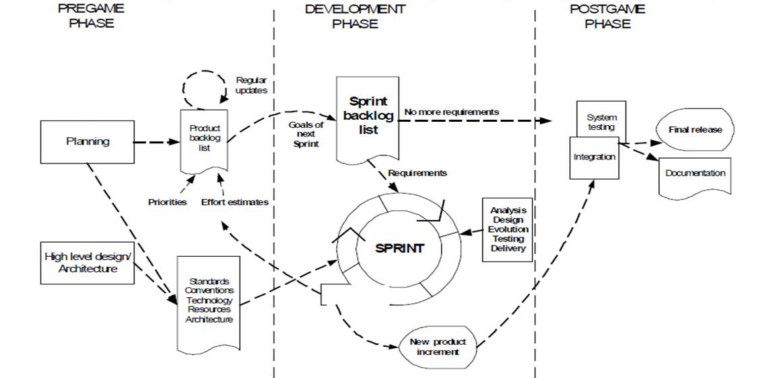
\includegraphics[scale=.8] {ScrumModel.png}
\caption{O Scrum como mostrado na figura acima é um quadro de gerenciamento de projetos de propósito geral que é aplicável a qualquer projeto com prazos agressivos com requisitos complexos e um grau de singularidade \cite{rees2002feasible}}
\label{fig:exampleFig5}
\end{figure}

O termo Scrum originalmente deriva de uma estratégia no jogo de rugby onde denota "obter uma bola fora de jogo de volta para o jogo" com o trabalho em equipe. O Scrum depende do auto-empenho, da auto-organização e da emergência em vez de medidas autoritárias. O Scrum é adequado para pequenas equipes de menos de 10 engenheiros. O processo Scrum inclui 3 fases: pré-jogo, desenvolvimento e pós-jogo.

A \textbf{fase pré-jogo} inclui 2 subfases:
    
A primeira subtarefa, denominada \textbf{planejamento} inclui a definição do sistema que está sendo desenvolvido. É criada uma lista de backlog de produtos contendo todos os requisitos conhecidos.

A segunda subtarefa denominada \textbf{arquitetura} trata o design de alto nível do sistema, incluindo a arquitetura e é planejada com base nos itens atuais no \textit{Product Backlog}.
    
Na \textbf{fase de desenvolvimento}, o sistema é desenvolvido em Sprints que são ciclos iterativos onde a funcionalidade é desenvolvida ou aprimorada para produzir novos incrementos. Cada Sprint inclui: Requisitos, Análise, Design, Evolução e fases de entrega.

A \textbf{fase pós-jogo} contém o encerramento do lançamento, incluindo tarefas como integração, testes de sistema e documentação. \cite{Kumar2014}


\subsection{Qualidade de Software}

Segundo a norma ISO 9000 (versão 2000), qualidade é "o grau em que um conjunto de características inerentes a um produto, processo ou sistema e cumpre os requisitos inicialmente estipulados para estes". Já \cite{Juran1998}, tem duas definições para qualidade "a característica dos produtos que atendem as necessidades dos clientes, e, assim, proporcionar a satisfação do mesmo" e "qualidade é a ausência de deficiências"

A definição específica sobre qualidade de software mais difundida é a encontrada nas normas ISO/EIC 9126-1 e ISO/IEC 25010, para as quais qualidade é "a capacidade do produto de software em satisfazer as necessidades implícitas e explícitas quando usado em condições específicas".

Para que o sistema possa atender as características de qualidade exigidas pela indústria automotiva, as especificações técnicas previstas na norma ISO/TS 16949 serão observadas. Esta norma especifica os requisitos do sistema da qualidade para a concepção, desenvolvimento, produção, instalação e manutenção de produtos automotivos e satisfaz a exigência da Volkswagen sobre os seus fornecedores.

\subsection{Práticas Engenharia de Software}

A Volkswagen espera que seus produtos estejam enquadrados em rígidos códigos de ética praticados no mercado. Desta maneira, para se alcançar este objetivo durante todo o processo, levaremos em consideração o trabalho desenvolvido por Simon Rogerson 2002 (The Software Engineering Code of Ethics and Professional Practice a case for being proactive), de maneira que possamos usufruir dos benefícios de suas recomendações, bem como estar em conformidade com as diretrizes da contratante. No artigo apresentado, daremos especial atenção à recomendação de produção de material bilingue, através de automação de procura de termos e eventuais traduções para os idiomas especificados. 

Com a finalidade de oferecer uma documentação de software de qualidade e tendo em mente os desafios desta tarefa, ainda mais em nossa língua portuguesa, e diante das características dos processos de desenvolvimento de softwares que em geral utilizam a língua inglesa, procuraremos gerenciar estes conflitos de idiomas através das recomendações do artigo de Christoph, Carlos e Fernando 2015 (Challenges in Analyzing Software Documentation in Portuguese). Com isto, procuraremos apresentar meios de documentar o software de maneira mais efetiva e eficaz para os interessados no processo.

Dada à característica da contratante, uma montadora de automóveis multinacional com necessidade de interação com equipes multiculturais ao redor do planeta, nosso objetivo será buscar um modelo sensível as diferentes culturas locais e seus desafios únicos. Para isto, tomaremos como base a publicação do painel de discussão de Rajesh e Vivek 2009 (Evolving Software Models for Global Organizations), que tem como objetivo discutir modelos que atendam às necessidades de organizações globais.

\subsection{Economia na Engenharia de Software}

De acordo com Jianglin, Hongyi e Yan-Fu 2015 (An Empirical Study of the Impact of Project Factors on Software Economics), tomaremos nossas decisões econômicas baseadas em quatro elementos importantes: produtividade, qualidade, esforço e “time-to-market”. Seguindo seus preceitos, poderemos contruir um relacionamento global das variáveis apresentadas. Como resultado deste processo proposto, alcançaremos melhores parâmetros quanto ao tamanho do time a ser empregado, o impacto em qualidade e produtividade da linguagem de programação a ser utilizada, a produtividade possível de ser alcançada e o tamanho previsto do software que poderá impactar diretamente no desenvolvimento e por consequência em sua data de entrega.

Como parâmetro decisório quanto ao julgamento de quando nosso software poderá ser considerado “bom o suficiente”, seguiremos o estudo de Susan e Joanne 2005 (Is My Software “Good Enough” to Release – A Probabilistic Assessment Methodology), o qual fornecerá subsídio para avaliarmos quando o mesmo estará pronto para entrega. A Fig.99 abaixo demonstra um modelo dos principais componentes representando atividades e artefatos identificados através de resultados experimentais publicados e literatura existente, os quais servirão como base para indicação efetiva da qualidade do software, seus processos para popular o modelo e métodos de análise de contribuições de evidências individuais que representaram a base para a conclusão de “Bom o Bastante para Entrega”, como apontado pelas autoras.

\begin{figure}[htp]
\centering
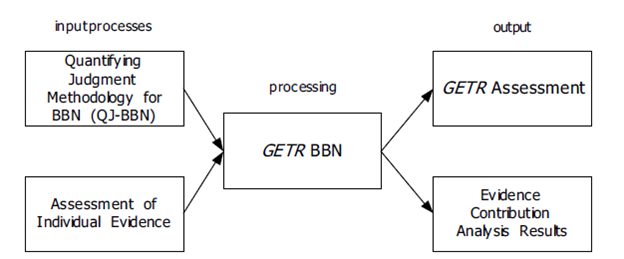
\includegraphics[scale=.8] {swebok_economia.png}
\caption{Componentes da Metodologia do “Bom o Bastante para Entrega”.}
\label{fig:exampleFig6}
\end{figure}

\bibliographystyle{ieeetr}
\bibliography{sbc-template}

%\bibliographystyle{sbc}
%\bibliography{sbc-template}



\end{document}
